\documentclass[Orbiter User Manual.tex]{subfiles} 
\begin{document}

\section{Introduction}

\begin{figure}[H]
  \centering
  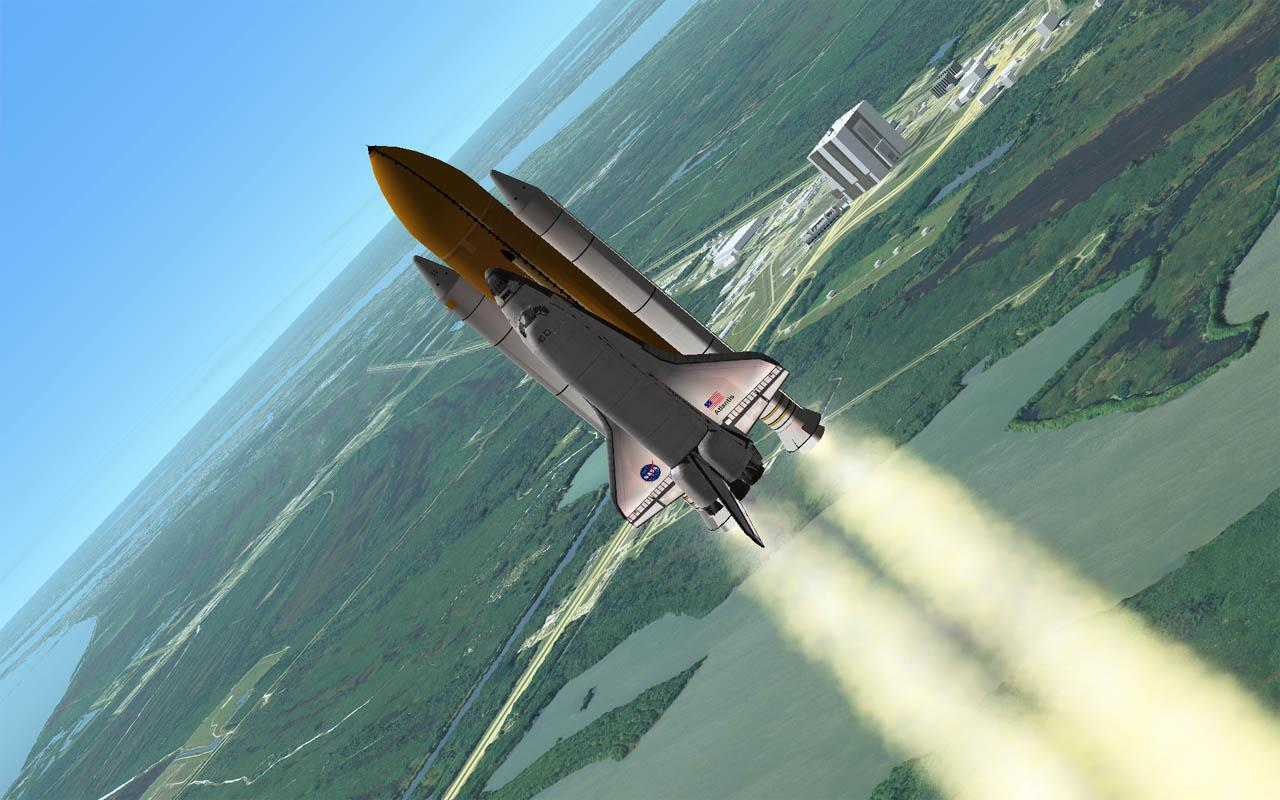
\includegraphics[width=0.99\hsize]{AtlantisLaunch.jpg}
\end{figure}

\textbf{Welcome to Orbiter 2016!}\\
\\
Orbiter 2016 is the latest instalment of the Orbiter Spaceflight simulator series. The most notable improvement from the 2010 Edition is the added support for surface elevation of planetary bodies, higher resolution surface and cloud textures, and improved surface collision modelling.\\
\\
High-resolution planetary texture packs are available for Earth, the Moon and Mars. In fact, there is now so much texture and elevation data available that you may need to free a bit of space on your hard disk to install it all – but I hope you'll agree that the result is worth the extra space.\\
\\
In addition, several of the spacecraft included in the standard distribution have had their cockpits updated and flight models improved. The simulation engine has been extensively reworked for improved stability.\\
\\
If the built-in graphics engine is not sufficient, Orbiter's interface for external graphics support has been extended. Try the excellent \textit{D3D9 Client} by Jarmo Nikkanen for advanced visual features and improved frame rates.\\
\\
As usual, the new version adds numerous bug fixes and feature enancements. Give it a try!\\
\\
\\
\textit{Martin Schweiger}



\subsection{About Orbiter}

They say a little knowledge is a dangerous thing, but it’s not one half so bad as a lot of ignorance.\\
\textit{Terry Pratchett – Equal Rites}\\
\\
Orbiter is a spaceflight simulator based on Newtonian mechanics. Its playground is our solar system with many of its major bodies – the sun, planets and moons. You take control of a spacecraft – either historic, hypothetical, or purely science fiction. Orbiter is unlike most commercial computer games with a space theme – there are no predefined missions to complete (except the ones you set yourself), no aliens to destroy and no goods to trade. Instead, you will get a pretty good idea about what is involved in real space flight – how to plan an ascent into orbit, how to rendezvous with a space station, or how to fly to another planet. It is more difficult, but also more of a challenge. Some people get hooked, others get bored. Finding out for yourself is easy – simply give it a try. Orbiter is free, so you don’t need to invest more than a bit of your spare time.\\
\\
Orbiter is a community project. The Orbiter core is just the skeleton that defines the rules of the simulated world (the \textit{physical model}). A basic solar system and some spacecraft (real and fictional) are included, but you can get a lot more with add-on modules developed by other enthusiasts in the Orbiter community. There are add-ons for nearly every spacecraft that ever flew (and quite a few that never got beyond the drawing board), for many more celestial bodies in the solar system (or entirely new fictional systems), for enhanced instruments, and much more. The Orbiter web site contains links to many Orbiter add-on repositories.

\subsection{About this manual}
This document is the main help file that comes with the basic distribution of Orbiter. It is a User’s Guide to the Orbiter software – which is to say that it gives an introduction into \textit{how} most things work, but doesn’t tell you much \textit{why} they behave as they do. By following the instructions, you will find out how to operate the engines of your spacecraft, how to use the instruments, and how to perform the most common missions.\\
\\
But a big part of the appeal of Orbiter is finding out about the \textit{why} – why do spacecraft in orbit behave as they do, what is involved in a gravity-assist flyby, why do rockets have multiple stages, why can it be tricky to line up for docking with a space station, what do the numbers in the instrument displays actually mean … ?\\
\\
This is where physics comes into the picture. If you want to conquer the final frontier, you will at some stage need to understand a few of the fundamental physical concepts that form the basis of astrodynamics and space flight. Luckily most of it is not very difficult – if you learn a bit about forces and gravity (“Newtonian mechanics”) and how they relate to the motion of planets and spacecraft in orbit (“Kepler’s laws”), you will have covered a good deal of it. Of course, there are always opportunities to dig deeper into the details, so your next steps might be finding out about the effects of orbit perturbations, attitude control, trajectory optimisation, mission planning, instrument design – to name just a few.\\
\\
Don’t get frustrated if you don’t succeed immediately – it’s only rocket science. Read the documentation and try some of the numerous Orbiter tutorials available on the internet, and you will soon be orbiting like a pro.\\
\\
Eventually you might start to develop your own add-on modules to enhance Orbiter’s functionality, write tutorials and help files for newcomers – or even take active part in the Orbiter core development by identifying and discussing flaws or omissions in the Orbiter physics model (and there are still many!)

\subsection{Orbiter on the web}
% TODO

\subsection{Finding more help}
% TODO

\subsection{Getting started}
% TODO

\end{document}
